%% LyX 2.3.4.3 created this file.  For more info, see http://www.lyx.org/.
%% Do not edit unless you really know what you are doing.
\documentclass[10pt,english,brazil]{beamer}
\usepackage[T1]{fontenc}
\usepackage[utf8]{inputenc}
\setcounter{secnumdepth}{3}
\setcounter{tocdepth}{3}
\usepackage{fancybox}
\usepackage{calc}
\usepackage{units}
\usepackage{textcomp}
\usepackage{amstext}
\usepackage{amsthm}
\usepackage{graphicx}
\usepackage[numbers]{natbib}
\PassOptionsToPackage{normalem}{ulem}
\usepackage{ulem}

\makeatletter
%%%%%%%%%%%%%%%%%%%%%%%%%%%%%% Textclass specific LaTeX commands.
% this default might be overridden by plain title style
\newcommand\makebeamertitle{\frame{\maketitle}}%
% (ERT) argument for the TOC
\AtBeginDocument{%
  \let\origtableofcontents=\tableofcontents
  \def\tableofcontents{\@ifnextchar[{\origtableofcontents}{\gobbletableofcontents}}
  \def\gobbletableofcontents#1{\origtableofcontents}
}
\theoremstyle{definition}
\newtheorem*{example*}{\protect\examplename}
\theoremstyle{plain}
\newtheorem*{prop*}{\protect\propositionname}

%%%%%%%%%%%%%%%%%%%%%%%%%%%%%% User specified LaTeX commands.
\usetheme{Warsaw}
\newtheorem{thm}{Teorema}[]
\newtheorem{cor}[]{Corollary}
\newtheorem{lem}[]{Lema}
\newtheorem{prop}[]{Proposi\c{c}\~ao}
\theoremstyle{definition}
\newtheorem{defn}[]{Definition}
\theoremstyle{remark}
\newtheorem{rem}[thm]{Remark}
\usepackage{amsthm}\usepackage{amsfonts}

\makeatother

\usepackage{babel}
\addto\captionsbrazil{\renewcommand{\examplename}{Exemplo}}
\addto\captionsbrazil{\renewcommand{\propositionname}{Proposição}}
\addto\captionsenglish{\renewcommand{\examplename}{Example}}
\addto\captionsenglish{\renewcommand{\propositionname}{Proposition}}
\providecommand{\examplename}{Exemplo}
\providecommand{\propositionname}{Proposição}

\begin{document}
\title{\selectlanguage{english}%
Métodos Estatísticos Básicos}
\subtitle{Aula 7 - Probabilidade condicional e independência}
\author{\selectlanguage{english}%
Prof. Regis Augusto Ely}
\institute{\selectlanguage{english}%
Departamento de Economia\\
Universidade Federal de Pelotas (UFPel)}
\date{\selectlanguage{english}%
Maio de 2014}
\makebeamertitle
\selectlanguage{brazil}%
\begin{frame}{Probabilidade condicional}

\begin{itemize}
\item Seja $(\Omega,\mathcal{A},P)$ um espaço de probabilidade. Se $B\in\mathcal{A}$
e $P(B)>0$, a \textit{\uline{probabilidade condicional}} de um
evento $A\in\mathcal{A}$ dado que o evento B ocorre, é definida por:

\shadowbox{\begin{minipage}[t]{0.4\columnwidth}%
$P(A|B)=\cfrac{P(A\cap B)}{P(B)}$.%
\end{minipage}}
\item Se $P(B)=0$, então $P(A|B)$ pode ser arbitrariamente definida. Podemos
usar $P(A|B)=0$ ou $P(A|B)=P(A)$.
\item Em termos de probabilidade frequentista:

\shadowbox{\begin{minipage}[t]{0.85\columnwidth}%
$P(A|B)=\underset{n\rightarrow\infty}{\lim}\cfrac{n\text{º de ocorrências de \ensuremath{A\cap B}em n ensaios}}{n\text{º de ocorrências de B nos mesmos n ensaios}}$.%
\end{minipage}}
\end{itemize}
\end{frame}

\begin{frame}{\foreignlanguage{english}{Probabilidade condicional}}

\begin{itemize}
\item Note que sempre que calcularmos $P(A|B)$ estamos calculando $P(A)$
em relação ao espaço amostral reduzido $B$.
\end{itemize}
\begin{center}
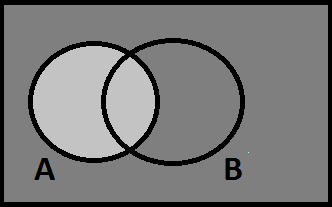
\includegraphics[scale=0.25]{1}
\par\end{center}

\begin{center}
$P(A)=\tfrac{\text{ Área de A}}{\text{ Área de \ensuremath{\Omega}}}$
\par\end{center}

\begin{center}
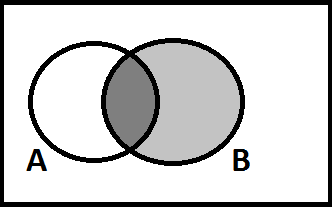
\includegraphics[scale=0.25]{2}
\par\end{center}

\begin{center}
$P(A|B)=\tfrac{\text{Área de \ensuremath{A\cap B}}}{\text{Área de B}}$
\par\end{center}

\end{frame}

\begin{frame}{\foreignlanguage{english}{Probabilidade condicional}}

\begin{example*}
$E=$ lançamos dois dados justos registrando o resultado como $(x_{1},x_{2})$.

Temos $\Omega=\begin{array}{cccc}
(1,1) & (1,2) & ... & (1,6)\\
(2,1) & (2,2) & ... & (2,6)\\
... & ... & ... & ...\\
(6,1) & (6,2 & ... & (6,6)
\end{array}$, com 36 resultados possíveis.

Dados os eventos: $A=\{(x_{1},$$x_{2})$| $x_{1}+x_{2}=10\}$ e $B=\{(x_{1},$$x_{2})$|
$x_{1}>x_{2}\}$.

\textbf{Calcule $P(A|B)$ e $P(B|A).$ }

Como $A=\{(5,5),(4,6),(6,4)\}$, e

$B=\{(2,1),(3,1),(3,2),(4,1),(4,2),(4,3),(5,1),(5,2),(5,3),...$

$...,(6,1),(6,2),(6,3),(6,4),(6,5)\}$

Temos $P(A)=\frac{3}{36}$ e $P(B)=\frac{15}{36}$. Logo, $P(A|B)=\frac{1}{15}$
e $P(B|A)=\frac{1}{3}$.

Alternativamente, como $P(A\cap B)=\frac{1}{36}$, temos $P(A|B)=\frac{P(A\cap B)}{P(B)}=\frac{\nicefrac{1}{36}}{\nicefrac{15}{36}}=\nicefrac{1}{15}$
e $P(B|A)=\frac{P(A\cap B)}{P(A)}=\frac{\nicefrac{1}{36}}{\nicefrac{3}{36}}=\frac{1}{3}$.
\end{example*}
\end{frame}

\begin{frame}{\foreignlanguage{english}{Probabilidade condicional}}

\selectlanguage{english}%
\begin{itemize}
\item Note que podemos calcular a probabilidade condicional \foreignlanguage{brazil}{\textbf{$P(A|B)$}}
de duas maneiras:
\end{itemize}
\selectlanguage{brazil}%
\begin{enumerate}
\item Calculando diretamente a probabilidade de A em relação ao espaço amostral
reduzido B;
\item Empregando a fórmula anterior, onde $P(A\cap B)$ e P(B) são calculados
em relação ao espaço amostral original $\Omega$.
\end{enumerate}
\begin{example*}
$E=$ retirar duas peças de um lote de 100 peças com 80 não-defeituosas
e 20 defeituosas, e observar os resultados.

$\Omega=\{(N,N),(N,D),(D,N),(D,D)\}$.

A = \{primeira peça é defeituosa\} e B = \{segunda peça é defeituosa\}.

Se extrairmos com reposição, $P(A)=P(B)=\frac{20}{100}=\frac{1}{5}$.

Sem repor a primeira peça, $P(B|A=D)=\frac{19}{99}$, ou $P(B|A=N)=\frac{20}{99}$.

Note que $P(B)=P(A=D)P(B|A=D)+P(A=N)P(B|A=N)=\frac{1}{5}.\frac{19}{99}+\frac{4}{5}.\frac{20}{99}=\frac{1}{5}$.
\end{example*}
\end{frame}

\begin{frame}{\foreignlanguage{english}{Partição do espaço amostral}}

\selectlanguage{english}%
\begin{itemize}
\item Dizemos que os eventos $B_{1},B_{2},...,B_{k}$ representam uma \textit{\uline{partição
do espaço amostral}} $\Omega$\foreignlanguage{brazil}{ quando:}
\end{itemize}
\selectlanguage{brazil}%
\begin{enumerate}
\item $B_{i}\cap B_{j}=\textrm{Ø},$ para todo $i\neq j$;
\item $\overset{k}{\underset{i=1}{\cup}}B_{i}=\Omega$;
\item $P(B_{i})>0$ para todo i.
\end{enumerate}
\begin{itemize}
\item Assim, quando o experimento $E$ é realizado, um, e somente um dos
eventos $B_{i}$ ocorre.
\end{itemize}
\begin{example*}
Ao jogar um dado e observar os resultados, os eventos $B_{1}=\{1,2\},$
$B_{2}=\{3,4,5\}$ e $B_{3}=\{6\}$ formam uma partição do espaço
amostral, enquanto $C_{1}=\{1,2,3,4\}$ e $C_{2}=\{4,5,6\}$ não formam.
\end{example*}
\end{frame}

\begin{frame}{Teorema da probabilidade total}

\selectlanguage{english}%
\begin{itemize}
\item Se os eventos $B_{1},B_{2},...,B_{k}$ formam uma partição do espaço
amostral $\Omega$, então podemos escrever qualquer evento $A\subseteq\Omega$
como $A=(A\cap B_{1})\cup(A\cap B_{2})\cup...\cup(A\cap B_{k})$.
\item Como os eventos dessas uniões são mutuamente excludentes, então $P(A)=P(A\cap B_{1})+P(A\cap B_{2})+...+P(A\cap B_{k}).$
\item Utilizando a fórmula da probabilidade condicional, obtemos o \textit{\uline{teorema
da probabilidade total:}}

\shadowbox{\begin{minipage}[t]{0.9\columnwidth}%
$P(A)=P(A/B_{1}).P(B_{1})+P(A/B_{2}).P(B_{2})+...+P(A/B_{k}).P(B_{k}).$%
\end{minipage}}
\end{itemize}
\end{frame}
\selectlanguage{brazil}%

\begin{frame}{\foreignlanguage{english}{Teorema de Bayes}}

\begin{itemize}
\item \textbf{Teorema de Bayes:} se $B_{1},B_{2},...,B_{k}$ formam uma
partição do espaço amostral $\Omega$, então 

\shadowbox{\begin{minipage}[t]{0.5\columnwidth}%
$P(B_{i}/A)=\cfrac{P(A/B_{i}).P(B_{i})}{\overset{k}{\underset{i=1}{\sum}}P(A/B_{i}).P(B_{i})}$.%
\end{minipage}}

\end{itemize}
\begin{example*}
{\footnotesize{}Problema de Monty-Hall: 3 portas e 1 prêmio. O apresentador
revela uma delas e pede se você quer trocar. A troca é vantajosa?
Considere os eventos}{\footnotesize\par}

{\footnotesize{}$A_{i}=$ \{prêmio está na porta i\} e $O=$ \{apresentador
revela porta 2\}. Temos}{\footnotesize\par}

{\footnotesize{}$P(A_{1})=P(A_{2})=P(A_{3})=\nicefrac{1}{3}$; $P(A_{1}|O)=\cfrac{P(A_{1}\cap O)}{P(O)}=\cfrac{P(O|A_{1})P(A_{1})}{P(O|A_{1})P(A_{1})+P(O|A_{2})P(A_{2})+P(O|A_{3})P(A_{3})}=\cfrac{\nicefrac{1}{2}.\nicefrac{1}{3}}{\nicefrac{1}{2}.\nicefrac{1}{3}+0+1.\nicefrac{1}{3}}=\cfrac{1}{3}$;
e}{\footnotesize\par}

{\footnotesize{}$P(A_{3}|O)=\cfrac{P(O|A_{3})P(A_{3})}{P(O)}=\cfrac{1.\nicefrac{1}{3}}{\nicefrac{1}{2}}=\cfrac{2}{3}$.
Logo, devemos trocar.}{\footnotesize\par}
\end{example*}
\end{frame}

\begin{frame}{\foreignlanguage{english}{Independência}}

\begin{itemize}
\item \textbf{Independência: }dado o espaço de probabilidade $(\Omega,\mathcal{A},P)$
, os eventos aleatórios A e B são independentes se, e somente se $P(A\cap B)=P(A).P(B).$
\item A independência entre A e B também equivale à $P(A|B)=P(A)$ e $P(B|A)=P(B)$,
porque $P(A\cap B)=P(A).P(B/A)=P(A).P(B)$. 
\item Se $P(A)=0$, então $P(A\cap B)=0,$ e A e B são independentes $\forall B\in\mathcal{A}$.
\item Se $P(B)=1$, então $P(A\cap B)=P(A)$, logo A e B são independentes
$\forall A\in\mathcal{A}$.
\end{itemize}
\begin{prop*}
O evento A é independente de si mesmo se, e somente se, $P(A)=0$
ou $P(A)=1$.
\end{prop*}
\begin{proof}
$P(A)=P(A\cap A)=P(A).P(A)\Leftrightarrow P(A)=0$ ou $P(A)=1$.
\end{proof}
\end{frame}

\begin{frame}{\foreignlanguage{english}{Independência}}

\begin{prop*}
Se A e B são eventos independentes, então A e $\bar{B}$ também são
(bem como $\bar{A}$ e B, e $\bar{A}$ e $\bar{B}$).
\end{prop*}
\begin{proof}
Sejam A e B eventos independentes. Como $A=(A\cap B)\cup(A\cap\bar{B})$,
então $P(A)=P(A\cap B)+P(A\cap\bar{B})$, de modo que $P(A\cap\bar{B})=P(A)-P(A\cap B)=P(A)-P(A).P(B)$
pela independência. Logo, $P(A\cap\bar{B})=P(A)(1-P(B))=P(A).P(\bar{B})$,
e $A$ e $\bar{B}$ são independentes.
\end{proof}
\begin{itemize}
\item A intuição por trás da proposição é a de que B é independente de A
se tanto a ocorrência quanto a não ocorrência de A não afetam a probabilidade
de B ocorrer, $P(B|A)=P(B)$ e $P(B|\bar{A})=P(B)$.
\item Se $A\cap B=\textrm{Ø}$, então A e B não são independentes (a menos
que um deles tenha probabilidade zero). Não confundir independência
com eventos excludentes ($P(A\cap B)=0$).
\end{itemize}
\end{frame}

\begin{frame}{Independência}

\begin{itemize}
\item Eventos aleatórios $A_{i}$ são independentes 2 a 2 se $P(A_{i}\cap A_{j})=P(A_{i}).P(A_{j})$,
$\forall i\neq j$.
\item Eventos $A_{1},...,A_{n}(n\geq2)$ são mutuamente independentes se
$P(A_{i1}\cap$$A_{i2}\cap$...$\cap A_{im})=P(A_{i1}).P(A_{i2})...P(A_{im})$,
$\forall1\leq i_{1}<i_{2}<...<i_{m}\leq n$, e $\forall n=2,3,...,n$.
\item Lembrar que a fórmula $P(A\cap B)=P(A).P(B)$ apenas se aplica quando
os eventos A e B são independentes, caso contrário devemos utilizar
a probabilidade condicional, $P(A\cap B)=P(A|B).P(B)$ (exemplo das
peças defeituosas).
\end{itemize}
\end{frame}

\begin{frame}{Indenpendência}

\begin{itemize}
\item Nem todos os eventos que são independentes 2 a 2 são mutuamente independentes.
\end{itemize}
\begin{example*}
$E=$ jogar dois dados e observar os resultados.

A = \{1º dado mostra nº par\}; B = \{2º dado mostra nº ímpar\};

C = \{ambos os dados mostram nº ímpares ou pares\}.

Temos $P(A)=P(B)=P(C)=\nicefrac{1}{2}$, e $P(A\cap B)=P(A\cap C)=P(B\cap C)=\nicefrac{1}{4}$,
mas $P(A\cap B\cap C)=0\neq P(A).P(B).P(C)$.
\end{example*}
\end{frame}

\end{document}
